\documentclass[tikz, border=10pt]{standalone}
\usepackage[T1]{fontenc}
\usepackage[utf8]{inputenc}
\usepackage{lmodern}
\usepackage[table]{xcolor}
\definecolor{IntelBlue}{HTML}{0068B5}
\definecolor{IntelLightBlue}{HTML}{DDEEF9}
\definecolor{FpgaOrange}{HTML}{E67E22}
\definecolor{FpgaLight}{HTML}{FDEBD0}
\definecolor{HpsGreen}{HTML}{1A7A4A}
\definecolor{HpsLight}{HTML}{D5F5E3}
\definecolor{GrayBg}{HTML}{F2F3F4}
\definecolor{GrayBorder}{HTML}{AAB7B8}
\definecolor{PassGreen}{HTML}{D5F5E3}
\definecolor{PassGreenDark}{HTML}{1E8449}
\definecolor{RowAlt}{HTML}{F7F9FB}
\definecolor{SummaryBg}{HTML}{EBF5FB}
\definecolor{NodeFill}{HTML}{D6EAF8}
\definecolor{NodeBorder}{HTML}{1B4F72}
\definecolor{InitFill}{HTML}{E5E7E9}
\definecolor{InitBorder}{HTML}{717D7E}
\definecolor{SleepFill}{HTML}{FEF5E7}
\definecolor{SleepBorder}{HTML}{935116}
\definecolor{MsgFill}{HTML}{D1F2EB}
\definecolor{MsgBorder}{HTML}{0E6655}
\definecolor{TimeoutRed}{HTML}{C0392B}
\definecolor{BtnBlue}{HTML}{1A5276}
\definecolor{ArrowGray}{HTML}{717D7E}
\usepackage{tikz}
\usetikzlibrary{shapes.geometric, arrows.meta, positioning, fit, backgrounds, calc, decorations.pathreplacing, bending, shadows.blur}
\begin{document}
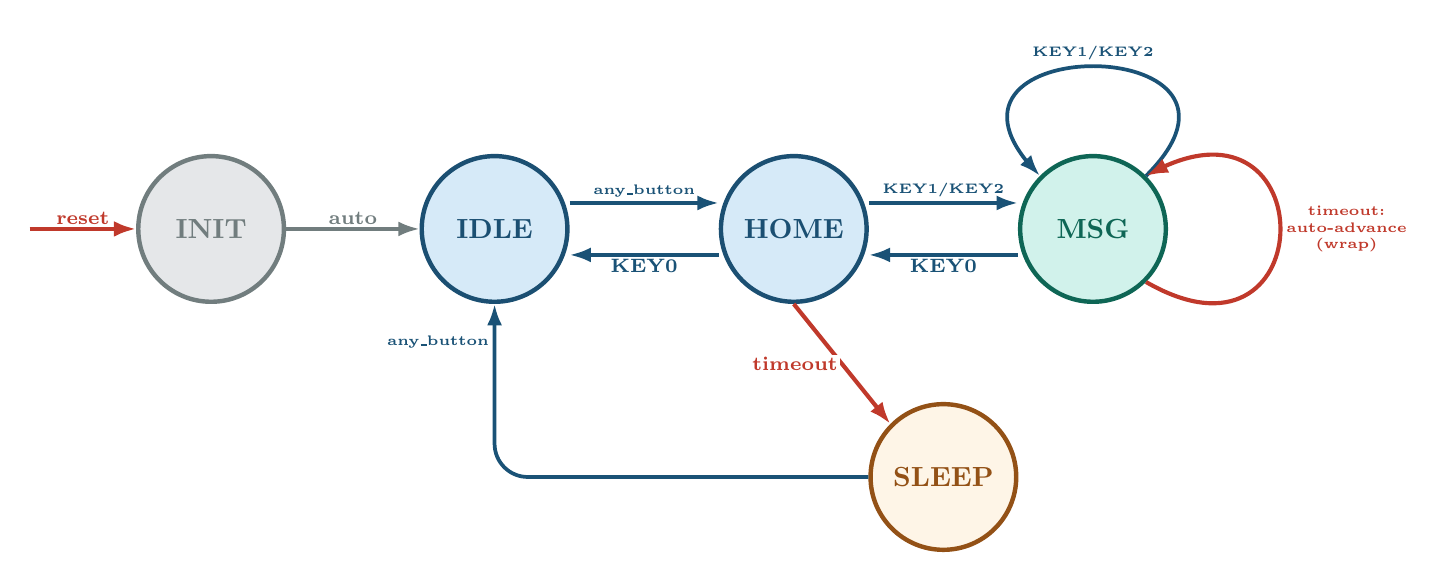
\begin{tikzpicture}[
  every node/.style={font=\sffamily},
  state/.style={circle, minimum size=1.85cm, line width=1.6pt,
                align=center, font=\normalsize\bfseries},
  initstate/.style={state, draw=InitBorder, fill=InitFill,
                    text=InitBorder},
  normalstate/.style={state, draw=NodeBorder, fill=NodeFill,
                      text=NodeBorder},
  msgstate/.style={state, draw=MsgBorder, fill=MsgFill,
                   text=MsgBorder},
  sleepstate/.style={state, draw=SleepBorder, fill=SleepFill,
                     text=SleepBorder},
  autoarr/.style={-{Latex[length=2.7mm,width=1.9mm]}, draw=ArrowGray,
                  line width=1.25pt},
  btnarr/.style={-{Latex[length=2.7mm,width=1.9mm]}, draw=BtnBlue,
                 line width=1.35pt},
  timeoutarr/.style={-{Latex[length=2.8mm,width=2.0mm]}, draw=TimeoutRed,
                     line width=1.5pt},
  lbl/.style={font=\scriptsize\bfseries, fill=white, inner sep=0.8pt},
  smalllbl/.style={font=\tiny\bfseries, inner sep=0.4pt}
]

\node[initstate]   (INIT)  at (0.0,  0.0) {INIT};
\node[normalstate] (IDLE)  at (3.6,  0.0) {IDLE};
\node[normalstate] (HOME)  at (7.4,  0.0) {HOME};
\node[msgstate]    (MSG)   at (11.2, 0.0) {MSG};
\node[sleepstate]  (SLEEP) at (9.3, -3.15) {SLEEP};

\draw[timeoutarr] ([xshift=-1.35cm]INIT.west) --
  node[lbl, above, text=TimeoutRed] {reset} (INIT.west);
\draw[autoarr] (INIT.east) --
  node[lbl, above, text=ArrowGray] {auto} (IDLE.west);

\draw[btnarr] ([yshift=0.33cm]IDLE.east) --
  node[smalllbl, above=1pt, text=BtnBlue] {any\_button}
  ([yshift=0.33cm]HOME.west);
\draw[btnarr] ([yshift=-0.33cm]HOME.west) --
  node[lbl, below, text=BtnBlue] {KEY0}
  ([yshift=-0.33cm]IDLE.east);

\draw[btnarr] ([yshift=0.33cm]HOME.east) --
  node[smalllbl, above=1pt, text=BtnBlue] {KEY1/KEY2}
  ([yshift=0.33cm]MSG.west);
\draw[btnarr] ([yshift=-0.33cm]MSG.west) --
  node[lbl, below, text=BtnBlue] {KEY0}
  ([yshift=-0.33cm]HOME.east);

\draw[btnarr] (MSG.north east)
  to[out=45, in=135, looseness=5.0]
  node[smalllbl, above=1pt, text=BtnBlue] {KEY1/KEY2}
  (MSG.north west);

\draw[timeoutarr] (HOME.south) --
  node[lbl, left, text=TimeoutRed] {timeout}
  (SLEEP.north west);
\draw[timeoutarr] (MSG.south east)
  to[out=-30, in=30, looseness=5.0]
  node[smalllbl, right=1pt, text=TimeoutRed, align=center]
       {timeout:\\auto-advance\\(wrap)}
  (MSG.north east);

\draw[btnarr, rounded corners=12pt]
  (SLEEP.west) -- (3.6,-3.15) --
  node[smalllbl, left=1pt, text=BtnBlue, pos=0.78] {any\_button}
  (IDLE.south);

\end{tikzpicture}
\end{document}
